\documentclass[10pt]{beamer}

\usepackage{listings}

\usepackage{wrapfig}

\usepackage{graphicx}
\graphicspath{ {../img/} }

\usepackage{fontspec}
\setmainfont{Ubuntu}[]
\setsansfont{Ubuntu}[]
\setmonofont{Ubuntu Mono}[]

\beamertemplatenavigationsymbolsempty

\lstset{
  language=ML,
  keywordstyle=\color{blue},
  backgroundcolor=\color{lightgray}
}

\title{Немного истории}

\begin{document}

\begin{frame}
  \frametitle{Немного истории}
  \textbf{Предыстория}: начало ХХ века.
  \par \bigskip
  \textbf{История Эрланг}: c 1985 по настоящее время.
  \par \bigskip
  \textbf{История Эликсир}: c 2012 по настоящее время.
\end{frame}


\begin{frame}
  \frametitle{Агнер Краруп Эрланг}
  \begin{wrapfigure}{l}{0.25\textwidth}
    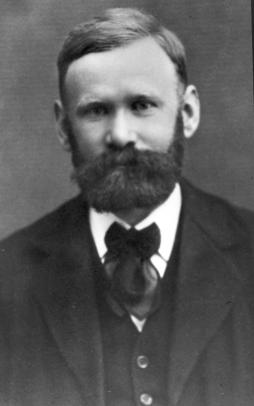
\includegraphics{agner_krarup_erlang}
  \end{wrapfigure}
  Датский математик, статистик и инженер.
  \par \bigskip
  Научный подход к изучению трафика в телефонных сетях.
  \par \bigskip
  Автор "Теории массового обслуживания".
\end{frame}

\begin{frame}
  \frametitle{Теория массового обслуживания}
  Она же теория очередей (Queueing theory).
  \par \bigskip
  Математическая модель для оценки пропускной способности телекоммуникационных сетей.
\end{frame}

\begin{frame}
  \frametitle{Теория массового обслуживания}
  применяется в телекоммуникационных системах,
  \par \bigskip
  и шире:
  \begin{itemize}
  \item в логистике,
  \item в управлении автомобильным движением,
  \item на конвейерном производстве,
  \item при проектировании складов и больниц.
  \end{itemize}
\end{frame}

\begin{frame}
  \frametitle{Эрланг}
  Родился в шведской компании Эрикссон (Ericsson).
  \par \bigskip
  Крупный поставщик телекомуникационного
  оборудования и услуг.
\end{frame}

\begin{frame}
  \frametitle{Эрланг}
  Для телеком индустрии характерны:
  \begin{itemize}
  \item сложное оборудование,
  \item сложный софт,
  \item большой трафик,
  \item жесткие требования по доступности сервиса.
  \end{itemize}
\end{frame}

\begin{frame}
  \frametitle{Ericsson’s Computer Science Laboratory}
  Задача найти более эффективные средства
  \par \bigskip
  разработки софта для железа и сервисов компании.
\end{frame}

\begin{frame}
  \frametitle{Ericsson’s Computer Science Laboratory}
  Прототипы телеком-приложений на разных языках:
  \begin{itemize}
  \item функциональные языки ML и Miranda,
  \item многопоточные языки ADA, Modula и Chill,
  \item логический язык Prolog,
  \item объектно-ориентированный Smalltalk.
  \end{itemize}
\end{frame}

\begin{frame}
  \frametitle{Ericsson’s Computer Science Laboratory}
  Ни один язык не имеет нужных возможностей.
  \par \bigskip
  Главная проблема -- многопоточность.
  \par \bigskip
  В итоге лаборатория решила
  разработать свой язык программирования.
\end{frame}

\begin{frame}
  \frametitle{Популярность Эрланг}
  2002 год, ejabberd -- первый крупный open source проект.
  \par \bigskip
  Стал основой для большинства IM (Instant Messaging) систем,
  \par \bigskip
  в т.ч. для широко известного WhatsApp.
\end{frame}

\begin{frame}
  \frametitle{Популярность Эрланг}
  2006 год, поддержка симметричной мультипроцессорности (SMP)
  \par \bigskip
  Эрланг научился эффективно использовать
  все имеющиеся в системе процессорные ядра.
\end{frame}

\begin{frame}
  \frametitle{Популярность Эрланг}
  У IT-индустрии появилась потребность
  разрабатывать многопоточные программы.
  \par \bigskip
  Возник интерес к функциональному программированию вообще,
  и к Эрланг в частности.
\end{frame}

\begin{frame}
  \frametitle{Интерес к ФП}
  Этот интерес проявился в двух направлениях:
  \begin{itemize}
  \item стали шире использоваться ФП языки;
  \item популярные языки начали заимствовать идеи ФП и реализовывать их у себя.
  \end{itemize}
\end{frame}

\begin{frame}
  \frametitle{Эликсир}
  Эликсир создан в 2012 году в компании Plataformatec.
  \par \bigskip
  Его автор -- Жозе Валим.
  \par \bigskip
  Один из основных разработчиков фреймворка Ruby on Rails
  и сооснователь компании Plataformatec.
\end{frame}

\begin{frame}
  \frametitle{Эликсир}
  Позаимствовал идеи из Ruby, Clojure и Эрланг.
  \par \bigskip
  Большое влияние Ruby и Ruby on Rails.
  \par \bigskip
  Система макросов заимствована из Clojure.
  \par \bigskip
  Унаследовал все возможности Эрланг и его виртуальной машины.
\end{frame}

\end{document}
